\newread\silofile%

\newcommand{\IfNonemptySiloFile}[3]{%
    \IfFileExists{#1}{%
        \openin\silofile=#1
        \ifeof\silofile%
            \closein\silofile%
            #3%
        \else
            \closein\silofile%
            #2%
        \fi
    }{%
        #3%
    }%
}

\newcommand{\SiloPlot}[3]{%
    \IfNonemptySiloFile{#3}{%
        \addplot+[#1]
        table [#2, col sep=comma] {#3};
    }{}%
}

\begin{figure*}[!t]
   \centering
    \begin{subfigure}[b]{0.33\linewidth}
    \begin{tikzpicture}[scale=0.875, transform shape]

        \begin{axis}[
            xlabel={Latency (\si{\micro\second})},
            ylabel={CCDF},
            xmode=normal,
            ymode=log,
            log basis y=10,
            ymin=1e-5,
            ymax=1,
            xmin=0,
            xmax=500,
            width={\linewidth},
            height=4.8cm,
            legend cell align=left,
            legend image post style={xscale=0.5},
            legend style={
                draw=none,
                font=\footnotesize,
                anchor=north east,
                at={(0.99, 1.41)},
                legend columns=2,
                /tikz/every even column/.append style={column sep=0.5cm},
            },
            xmajorgrids=true,
            ymajorgrids=true,
            yminorgrids=true,
        ]
        \addplot[ultra thick, cRed!70, dashed] table [x=latency_us, y=ccdf, col sep=comma] {data/silo_ccdf_downsampled_Delivery.csv};
        \addlegendentry{Delivery}

        \addplot[ultra thick, cViolet!80, dashed] table [x=latency_us, y=ccdf, col sep=comma] {data/silo_ccdf_downsampled_StockLevel.csv};
        \addlegendentry{StockLevel}

        \addplot[ultra thick, cYellow, solid] table [x=latency_us, y=ccdf, col sep=comma] {data/silo_ccdf_downsampled_all.csv};
        \addlegendentry{Overall}

        \addplot[ultra thick, cGreen!80, dashed] table [x=latency_us, y=ccdf, col sep=comma] {data/silo_ccdf_downsampled_NewOrder.csv};
        \addlegendentry{NewOrder}

        \addplot[ultra thick, cBlue!80, dashed] table [x=latency_us, y=ccdf, col sep=comma] {data/silo_ccdf_downsampled_Payment.csv};
        \addlegendentry{Payment}

        \addplot[ultra thick, gray!80, dashed] table [x=latency_us, y=ccdf, col sep=comma] {data/silo_ccdf_downsampled_OrderStatus.csv};
        \addlegendentry{OrderStatus}
        \end{axis}
    \end{tikzpicture}
    \caption{CCDF of task execution time}
    \label{sfig:silo_ccdf}
    \end{subfigure}
    \begin{subfigure}[b]{0.33\linewidth}
    \begin{tikzpicture}[scale=0.875, transform shape]
        \begin{axis}
            [
            xlabel={Load (KQPS)},
            ylabel={Latency (us)},
            legend style={draw=none},
            xmin=0,
            ymin=0,
            xmax=400,
            ymax=1000,
            restrict x to domain*=0:5E9,
            restrict y to domain*=0:1E4,
            axis y line=left,
            axis x line=bottom,
            width={\linewidth},
            height=4.25cm,
            legend cell align=left,
            legend image post style={xscale=0.6},
            legend style={
                draw=none,
                fill=none,
                font=\footnotesize,
                anchor=north east,
                at={(1.00, 1.71)},
                legend columns=2,
                /tikz/every even column/.append style={column sep=0.4cm},
                },
            ]

            \addlegendimage{kcmStyle}
            \addlegendentry{KCM}

            \addlegendimage{partitionStyle}
            \addlegendentry{TCP-CP-80}

            \addlegendimage{floating_tlsStyle}
            \addlegendentry{TCP-CS-80 TLS}

            \addlegendimage{floatingStyle}
            \addlegendentry{TCP-CS-80}

            \addlegendimage{workerPool_tlsStyle}
            \addlegendentry{Worker Pool TLS}

            \addlegendimage{workerPoolStyle}
            \addlegendentry{Worker Pool}

            \addlegendimage{koma_tlsStyle}
            \addlegendentry{\system-kTLS}

            \addlegendimage{komaStyle}
            \addlegendentry{\system}

            \SiloPlot{
                partitionStyle,
                x filter/.code={
                    \IfStrEq{\thisrow{dist_config}}{silo}{}{\def\pgfmathresult{}}
                }
            }{x expr=\thisrow{load_silo-partition(QPS)} / 1000, y=latency_silo-partition}{data/silo_bench.csv}

            \SiloPlot{
                komaStyle,
                x filter/.code={
                    \IfStrEq{\thisrow{dist_config}}{silo}{}{\def\pgfmathresult{}}
                }
            }{x expr=\thisrow{load_silo-koma(QPS)} / 1000, y=latency_silo-koma}{data/silo_bench.csv}

            \SiloPlot{
                floatingStyle,
                x filter/.code={
                    \IfStrEq{\thisrow{dist_config}}{silo}{}{\def\pgfmathresult{}}
                }
            }{x expr=\thisrow{load_silo-floating(QPS)} / 1000, y=latency_silo-floating}{data/silo_bench.csv}

            \SiloPlot{
                workerPoolStyle,
                x filter/.code={
                    \IfStrEq{\thisrow{dist_config}}{silo}{}{\def\pgfmathresult{}}
                }
            }{x expr=\thisrow{load_silo-pool(QPS)} / 1000, y=latency_silo-pool}{data/silo_bench.csv}

            \SiloPlot{
                kcmStyle,
                x filter/.code={
                    \IfStrEq{\thisrow{dist_config}}{silo}{}{\def\pgfmathresult{}}
                }
            }{x expr=\thisrow{load_silo-kcm_floating(QPS)} / 1000, y=latency_silo-kcm_floating}{data/silo_bench.csv}

            \SiloPlot{
                floating_tlsStyle,
                x filter/.code={
                    \IfStrEq{\thisrow{dist_config}}{silo}{}{\def\pgfmathresult{}}
                }
            }{x expr=\thisrow{load_silo-floating-tls(QPS)} / 1000, y=latency_silo-floating-tls}{data/silo_tls.csv}

            \SiloPlot{
                workerPool_tlsStyle,
                x filter/.code={
                    \IfStrEq{\thisrow{dist_config}}{silo}{}{\def\pgfmathresult{}}
                }
            }{x expr=\thisrow{load_silo-pool-tls(QPS)} / 1000, y=latency_silo-pool-tls}{data/silo_tls.csv}

            \SiloPlot{
                koma_tlsStyle,
                x filter/.code={
                    \IfStrEq{\thisrow{dist_config}}{silo}{}{\def\pgfmathresult{}}
                }
            }{x expr=\thisrow{load_silo-koma-tls(QPS)} / 1000, y=latency_silo-koma-tls}{data/silo_tls.csv}
        \end{axis}
    \end{tikzpicture}
    \caption{\nineninepct latency vs. throughput}
    \label{sfig:silo_bench}
\end{subfigure}
\begin{subfigure}[b]{0.33\linewidth}
\centering

\begin{subfigure}[b]{\linewidth}
\begin{tikzpicture}[scale=0.875, transform shape]
\begin{axis}
    [
    ylabel={Latency (us)},
    legend style={draw=none},
    xmin=0,
    ymin=0,
    xmax=180,
    ymax=2000,
    axis y line=left,
    axis x line=bottom,
    height=2.9cm,
    width={\linewidth},
    legend cell align=left,
    legend image post style={xscale=0.6},
    legend style={
        draw=none,
        fill=none,
        font=\footnotesize,
        anchor=north east,
        at={(1.20, 1.80)},
        legend columns=2,
        /tikz/every even column/.append style={column sep=0.4cm},
        },
    ]

            \addlegendimage{grpc_vanillaStyle, dotted, mark=*, cLightPurple!80}
            \addlegendentry{gRPC-POSIX-24}

            \addlegendimage{grpc_komaStyle, dotted, mark=*, cViolet!80}
            \addlegendentry{grpc-\system-24}

            \addlegendimage{grpc_vanillaStyle}
            \addlegendentry{gRPC-POSIX-5,000}

            \addlegendimage{grpc_komaStyle}
            \addlegendentry{grpc-\system-5,000}

\SiloPlot{grpc_komaStyle, dotted, mark=*, mark size=0.8pt}{x expr=\thisrow{load_silo-grpc-koma-go(QPS)}/1000, y=latency_silo-grpc-koma-go}{data/silo_grpc_24conn.csv}
\SiloPlot{grpc_vanillaStyle, dotted, mark=*, mark size=0.8pt}{x expr=\thisrow{load_silo-grpc-go(QPS)}/1000, y=latency_silo-grpc-go}{data/silo_grpc_24conn.csv}
\end{axis}
\end{tikzpicture}
\end{subfigure}

\vspace{-2pt}

\begin{subfigure}[b]{\linewidth}
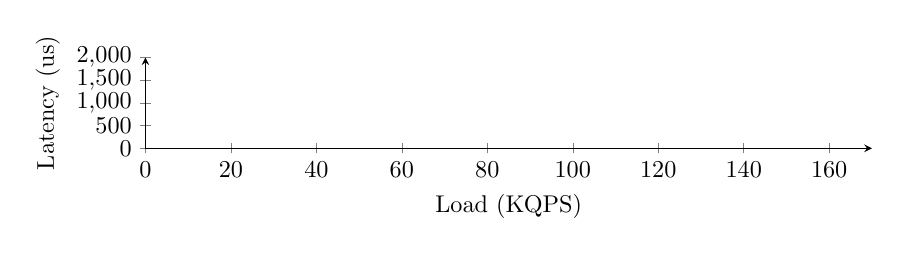
\begin{tikzpicture}[scale=0.875, transform shape]
\begin{axis}
    [
    xlabel={Load (KQPS)},
    ylabel={Latency (us)},
    legend style={draw=none},
    xmin=0,
    ymin=0,
    xmax=170,
    ymax=2000,
    restrict x to domain*=0:5E9,
    restrict y to domain*=0:1E4,
    axis y line=left,
    axis x line=bottom,
    height=2.9cm,
    width={\linewidth},
    legend cell align=left,
    legend image post style={xscale=0.6},
    legend style={
        draw=none,
        fill=none,
        font=\footnotesize,
        anchor=north east,
        at={(1.00, 1.37)},
        legend columns=2,
        /tikz/every even column/.append style={column sep=0.4cm},
        },
    ]
\SiloPlot{grpc_komaStyle}{x expr=\thisrow{load_silo-grpc-koma-go(QPS)}/1000, y=latency_silo-grpc-koma-go}{data/silo_grpc_5000conn.csv}
\SiloPlot{grpc_vanillaStyle}{x expr=\thisrow{load_silo-grpc-go(QPS)}/1000, y=latency_silo-grpc-go}{data/silo_grpc_5000conn.csv}
\end{axis}
\end{tikzpicture}
\end{subfigure}
\caption{\nineninepct latency vs. throughput}
\label{sfig:silo_grpc}
\end{subfigure}

\caption{Silo running TPC-C benchmark.}
\label{fig:silo}
\end{figure*}
